%!TEX root = ../main.tex

\graphicspath{{./figures/chapter5/}}

\chapter{RNA localization by the numbers}
\label{ch:chapter5}

\minitoc
\newpage

In this chapter, I present several applications of the pipeline described in the previous chapters.
More specifically, I analyze experimental datasets in order to explore, quantify and validate biological insights about \ac{mRNA} localization.
Results from this chapter are computed from three different high content screening studies, totaling tens of transcripts observed through thousands of bioimages.

In the first section, I develop a general classification pipeline to identify generic \ac{mRNA} localization patterns from \ac{smFISH} images~\cite{CHOUAIB_2020}.
In the second section, exploiting the same dataset, I focus on a specific and novel clustering pattern: the translation factories.
These first two sections describe the work published in:

\begin{center}
	\color{green}
	R. Chouaib, A. Safieddine, et al. (2020), \textit{A dual protein-mRNA localization screen reveals compartmentalized translation and widespread co-translational RNA targeting}, Developmental Cell 54 (6), 773.
\end{center}

In the third section, I exploit a \ac{GFP} channel to visualize and detect centrosomes.
I observed a centrosomal localization patterns for different transcripts and mitosis phases~\cite{safieddine_choreography_2021}.
This work was published in:

\begin{center}
	\color{green}
	A. Safieddine, E. Coleno, et al. (2021), \textit{A choreography of centrosomal mRNAs reveals a conserved localization mechanism involving active polysome transport}, Nature Communications 12 (1), 1352.
\end{center}

In the fourth section, I detail several transcripts with a protrusion localization pattern~\cite{pichon_kinesin_2021}.
This last section mainly describes results presented in:

\begin{center}
	\color{green}
	X. Pichon, K. Moissoglu, et al. (2021), \textit{The kinesin KIF1C transports APC-dependent mRNAs to cell protrusions}, RNA 27 (12), 1528.
\end{center}

\section{A systemic quantification of RNA localization}
\label{sec:general_pattern_recognition}

In~\cite{CHOUAIB_2020}, I have implemented a quantitative pipeline to analyze the localizations of \ac{mRNA} molecules.
This work lays the foundation of the future Python packages developed in FISH-quant V2~\cite{Imbert_fq_2022}.
My contribution consists in classifying individual cells with one or several \ac{RNA} localization patterns.

\subsection{Introduction}
\label{subsec:introduction_general_pattern}

Most of \ac{mRNA}s have a random distribution throughout the cytoplasm, but some of them localize in specific subcellular regions.
This phenomenon has been previously reviewed in different papers~\cite{Blower_2013, Jung_2014, Eliscovich_2017, Bovaird_2018}.

Such localization can be related to either the \ac{RNA} metabolism, for example with untranslated \ac{mRNA}s stored and repressed in \ac{P-bodies} (but not degraded~\cite{Hubstenberger_2017}), or the protein metabolism with locally translated proteins.
This local synthesis concerns both mature proteins and nascent peptides.
Different cellular processes imply the delivery of mature proteins in specific subcellular regions and a local regulation of the proteome.
Local translation can contributes to cell fate determination during metazoan development, as observed in~\cite{melton_translocation_1987} with a clear modification of the Vg1 \ac{RNA} spatial distribution between mature and immature Xenopus oocytes.
In these same Xenopus embryos, cyclin B1 \ac{mRNA}s localized at the mitotic apparatus could also play an important role in the rapid cell division cycles observed during early embryogenesis~\cite{Groisman_2000}.
In mammal cells, \ac{RNA} localization influences cell polarization and motility, usually through actin localization at the cell edge~\cite{Lawrence_1986}.
Locally translated proteins are also known to be involved in axonal growth and so neural plasticity~\cite{VanDriesche_2018}.
Finally, by precisely controlling the \ac{mRNA} localization and the subsequent translation process, cells can avoid to release proteins at inappropriate places~\cite{Muller_myelin_2013} and help the synthesis of protein complexes~\cite{pichon_visualization_2016}.

Several mechanisms will drive the localization of \ac{mRNA}s.
Sometimes the nascent peptide can serve as a targeting signal, but most of the time the \ac{RNA} molecule itself will initiate its localization.
\ac{RNA} can also be trapped in specific subcellular compartments.
The molecule often include a zip-code sequence that is read by a \ac{RBP} and starts the assembly of a transport complex comprising different organelles or motor proteins.
Such complex can then directly convey the \ac{RNA} along the cytoskeleton~\cite{Blower_2013}.
Coupled with an anchoring mechanism at the targeted destination, it provides a better stability of the \ac{RNA} localization.

In~\cite{CHOUAIB_2020}, we claim that a global view of local translation in the whole cell and at the genomic level is still to come, despite recent progress.
In a pioneering work on Drosophila embryogenesis~\cite{lecuyer_global_2007}, authors analyze 3,370 genes and find that 71\% of them encode a transcript with a non-uniform localization pattern.
In human cell lines recent studies exploit and improve \ac{smFISH} techniques to image thousands of \ac{mRNA}s in the perinuclear region, the mitochondria and the cell membrane~\cite{battich_image-based_2013, Chen_2015, eng_seqfish_2019, Xia_2019}.
We take a step forward in studying \ac{mRNA} localization with human cell lines and a systematic approach.
We perform a quantitative analysis leveraging supervised and unsupervised methods in order to recognize up to 6 different localization patterns.
The current section emphasizes this quantitative pipeline that contributes to make our analysis scalable and more robust.

\subsection{Materials and methods}
\label{subsec:materials_general_pattern}

The quantitative pipeline used in this study and the existing work in FISH-quant V1 are the building blocks of FISH-quant V2.
Therefore, the various methods presented here were not yet packaged in \emph{bigfish}, but Python libraries that formed its foundation were already in used.
This work is developed in Python and the code repository is public\footnote{\url{https://github.com/Henley13/paper_translation_factories_2020}}.

\subsubsection{Experimental data}

At first more than 500 genes have been manually analyzed to identify potential transcripts with non random localization patterns within the cell.
In addition to different qualitative and manual observations performed over this dual \ac{RNA}-protein localization screen, we also develop a quantitative pipeline to systematically classify transcripts' localization patterns.
To this end, I exploit a dataset of 526 \ac{FoV}s, combining DAPI and \ac{smFISH} channels as illustrated in Figure~\ref{fig:fov_racha}.
The raw images stacks several 2D acquisitions to gather a 3D information of the \ac{FoV} with a z-spacing of 0.3μm.
Acquisitions are performed with a Zeiss Axioimager Z1 widefield microscope or a Nikon Ti fluorescence microscope, on human cell lines HeLa.
In total, this dataset is built from 57 independent experiments gathering observations from 27 different \ac{mRNA}s under different experimental conditions.

\begin{figure}[]
    \centering
    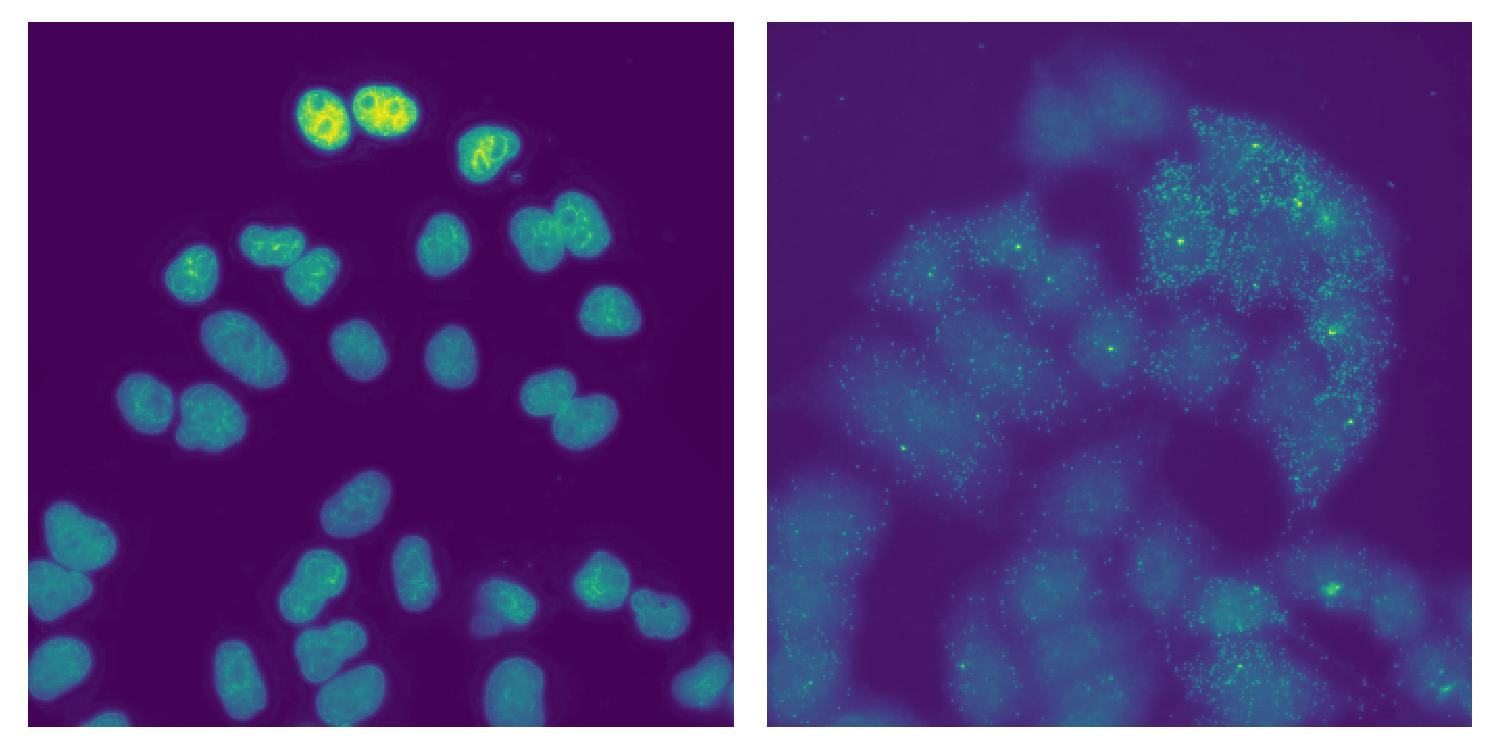
\includegraphics[width=\textwidth]{figures/chapter5/FoV_DYNLL2}
    \caption[Contrasted image with Dapi and smFISH channels]{Contrasted image with Dapi (\textit{left}) and smFISH (\textit{right}) channels.
	Images are projected in 2D.
	Targeted transcript is DYNLL2.
	Plot built with \emph{bigfish}}
    \label{fig:fov_racha}
\end{figure}

\subsubsection{Semi-automated RNA detection}

\ac{RNA} detection is performed with a Python implementation of FISH-quant v1~\cite{mueller_fish-quant_2013}.
I apply a \ac{LoG} filter on the 3D \ac{smFISH} images, then a local maximum detection algorithm.
However, a threshold value has to be set manually for every experiment to discriminate the actual spots from the noisy background blobs.
Large agglomeration of spots are decomposed with a gaussian mixture model, following~\cite{samacoits_computational_2018}.
Ultimately, \ac{RNA} clusters - namely foci - are detected with a DBSCAN algorithm~\cite{ester_density-based_1996} applied on the detected spots.
According to the way a DBSCAN cluster samples, a foci is then defined as a set of at least 5 points where for each point there is at least one other point from the foci within a 350 nanometers distance.
All foci overlapping the nuclear area in the projected 2D images are considered as a transcription site and removed from the analysis.
Percentages of \ac{RNA} in foci are then calculated as number of \ac{RNA} inside the cytoplasmic foci divided by the number of cytoplasmic \ac{RNA}s.

There are two main differences compared to the current detection methods implemented in FISH-quant and presented in Chapter~\ref{ch:chapter2}: a detection threshold has to be set manually and the decomposition of agglomerated spots has since been simplified.

\subsubsection{Cell and nucleus segmentation}

Nucleus segmentation is performed from the DAPI channel and cell segmentation from the cell autofluorescence in the \ac{smFISH} channel.
Segmentation is performed in 2D for both nuclei and cells, thus 3D images are projected in two dimensions using their maximal local focus values~\cite{tsanov_smifish_2016}.

Nuclei are segmented with NucleAIzer~\cite{hollandi_nucleaizer_2020}, a deep neural network pipeline trained with the annotations from the Data Science Bowl 2018 challenge\footnote{\url{https://www.kaggle.com/c/data-science-bowl-2018}}.
This pipeline is based on a Mask R-CNN architecture~\cite{He_2017_ICCV}, with optionally a fine-tuning of the segmented boundaries with a U-Net model~\cite{Ronneberger_unet}.
After a first round of segmentation, some nuclei are missing, so I remove the segmented nuclei from the DAPI channel and feed NucleAIzer with the remaining nuclei for a second round of segmentation.
Removing the segmented nuclei from the original image implies some morphological mathematics techniques as described in Chapter~\ref{ch:chapter3}.
This technique is now implemented in FISH-quant.

Cells are segmented with a watershed algorithm using nucleus masks as seeds.
A threshold value is set manually for every experiment to discriminate the cell surface from the background.
In case of poor results, some segmentation masks are corrected manually.
This is especially the case for transcript that tend to localize in cell protrusion.
Indeed, such localization pattern is highly sensitive to the segmentation accuracy.

\subsubsection{Localization feature engineering}

Based on the segmentation masks and the coordinates of the detected spots, I identify 9,710 individual cells with an average of 346 \ac{RNA}s per cell.
For each cell, I collect the cell and nucleus masks in 2D, the \ac{RNA} and the potential cluster coordinates in 3D.
In addition I save an image of the cell, for visualization purpose, and different information about the experiment (the presence of a treatment, the targeted gene, etc.).
Cropped cells, empty cells or cells with less than 30 detected \ac{RNA} inside are removed.
At this point, I have a coordinate representation of every cell, as presented in Chapter~\ref{ch:chapter4}.

I design and compute a set of 15 features to describe the spatial distribution of points inside the cell:
\begin{itemize}
	\setlength\itemsep{0.1em}
	\item The number of foci.
	\item The proportion of \ac{RNA} inside foci.
	\item The proportion of \ac{RNA} inside the nucleus.
	\item The average \ac{RNA} distance to the cell membrane, normalized by the value obtained under a uniform \ac{RNA} distribution.
	\item The average \ac{RNA} distance to the nucleus membrane, normalized by the value obtained under a uniform \ac{RNA} distribution.
	\item The average foci distance to the cell membrane, normalized by the value obtained under a uniform foci distribution.
	\item The average foci distance to the nucleus membrane, normalized by the value obtained under a uniform foci distribution.
	\item The proportion of \ac{RNA} inside cell protrusion.
	A protrusion region is defined by calculating the difference between the segmented cellular region and its morphological opening with a large window.
	\item The peripheral dispersion index, defined as the squared point distance to the centroid of the cell and normalized by the value obtained under a uniform \ac{RNA} distribution.
	\item The number of \ac{RNA}s within 515 nm from the nucleus membrane, normalized by the value obtained under a uniform \ac{RNA} distribution.
	\item The number of \ac{RNA}s between 515 nm and 1030 nm from the nucleus membrane, normalized by the value obtained under a uniform \ac{RNA} distribution.
	\item The number of \ac{RNA}s between 1030 nm and 1545 nm from the nucleus membrane, normalized by the value obtained under a uniform \ac{RNA} distribution.
	\item The number of \ac{RNA}s between 0 nm and 515 nm from the cell membrane, normalized by the value obtained under a uniform \ac{RNA} distribution.
	\item The number of \ac{RNA}s between 515 nm and 1030 nm from the cell membrane, normalized by the value obtained under a uniform \ac{RNA} distribution.
	\item The number of \ac{RNA}s between 1030 nm and 1545 nm from the cell membrane, normalized by the value obtained under a uniform \ac{RNA} distribution.
\end{itemize}

The apparent precision of the nanometer distances is just an artifact as the concentric regions are delimited visually from a sample of cell images.
Therefore, the width of these regions are defined in pixels, more precisely, with a 5 pixels width and a pixel size of 103 nm.

\subsubsection{Binary classification models}

\begin{figure}[]
	\centering
	\minipage{0.2\textwidth}
		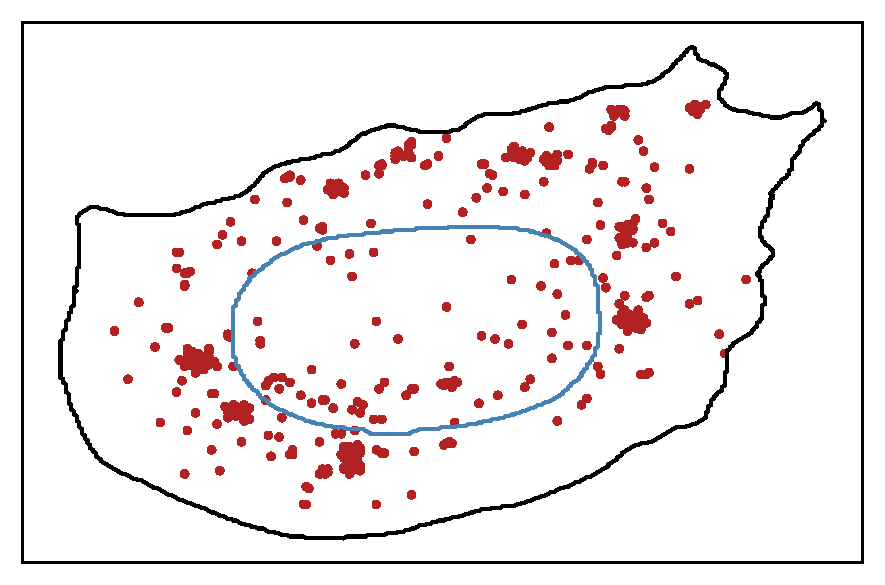
\includegraphics[trim={0.5cm 0.5cm 0.5cm 0.5cm},clip,width=\linewidth]{figures/chapter5/plot_foci}
		\subcaption{Foci}
	\endminipage\hfill
	\minipage{0.2\textwidth}
		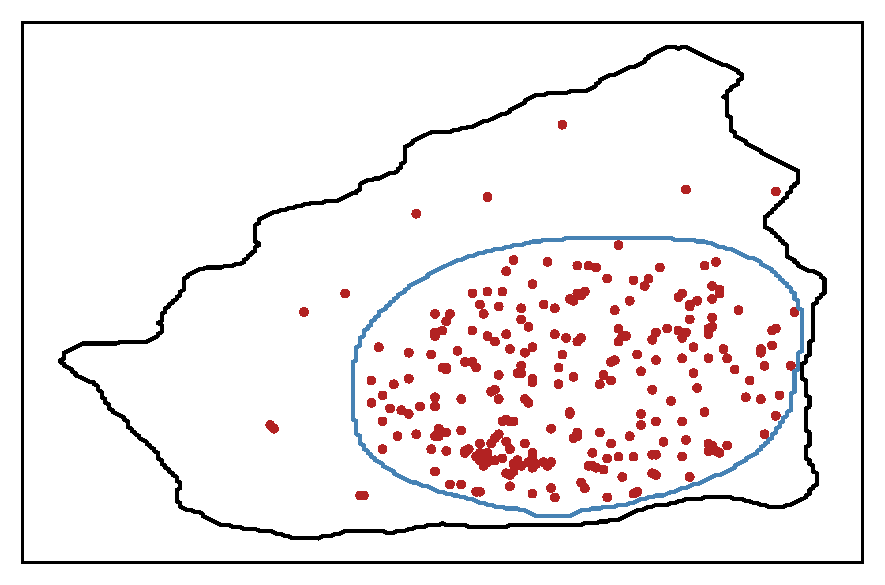
\includegraphics[trim={0.5cm 0.5cm 0.5cm 0.5cm},clip,width=\linewidth]{figures/chapter5/plot_intranuclear}
		\subcaption{Intranuclear}
	\endminipage\hfill
	\minipage{0.2\textwidth}
		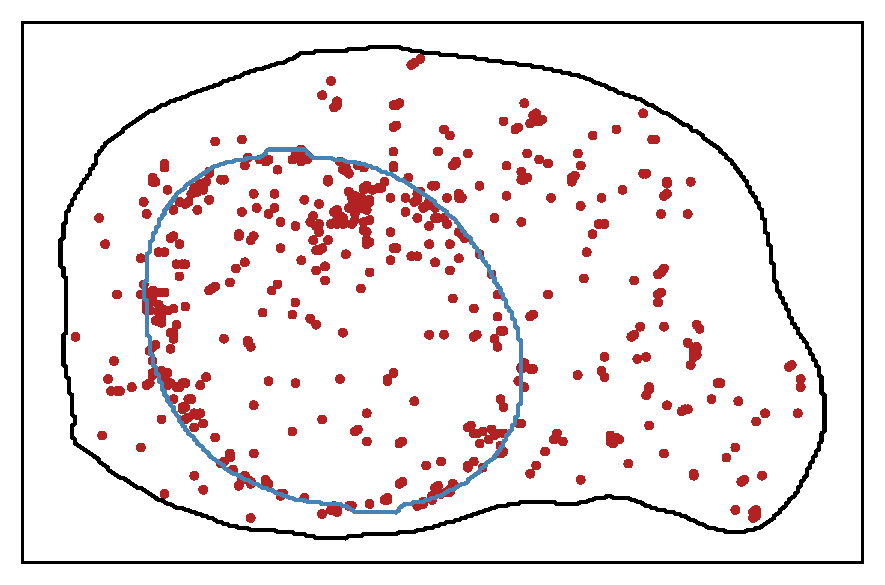
\includegraphics[trim={0.5cm 0.5cm 0.5cm 0.5cm},clip,width=\linewidth]{figures/chapter5/plot_nuclear}
		\subcaption{Nuclear edge}
	\endminipage\hfill
	\minipage{0.2\textwidth}
		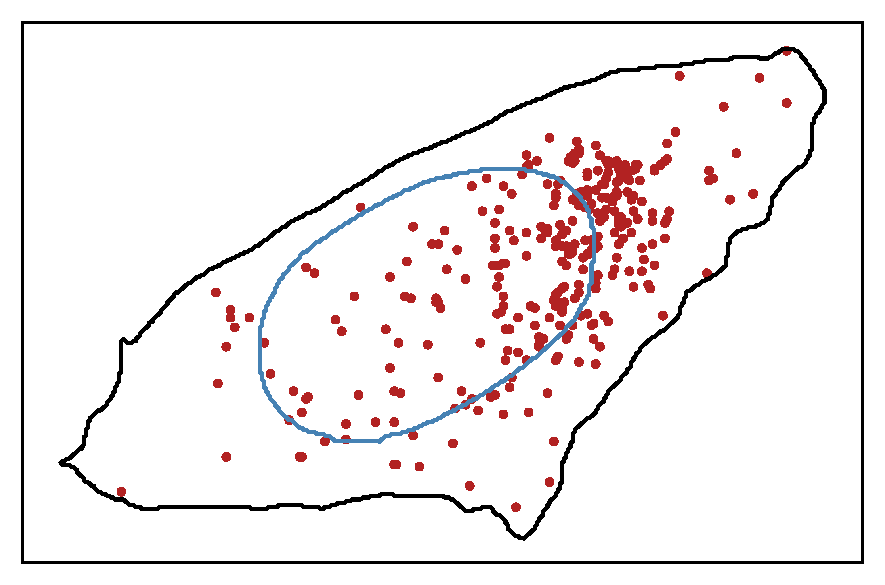
\includegraphics[trim={0.5cm 0.5cm 0.5cm 0.5cm},clip,width=\linewidth]{figures/chapter5/plot_perinuclear}
		\subcaption{Perinuclear}
	\endminipage\hfill
	\minipage{0.2\textwidth}
		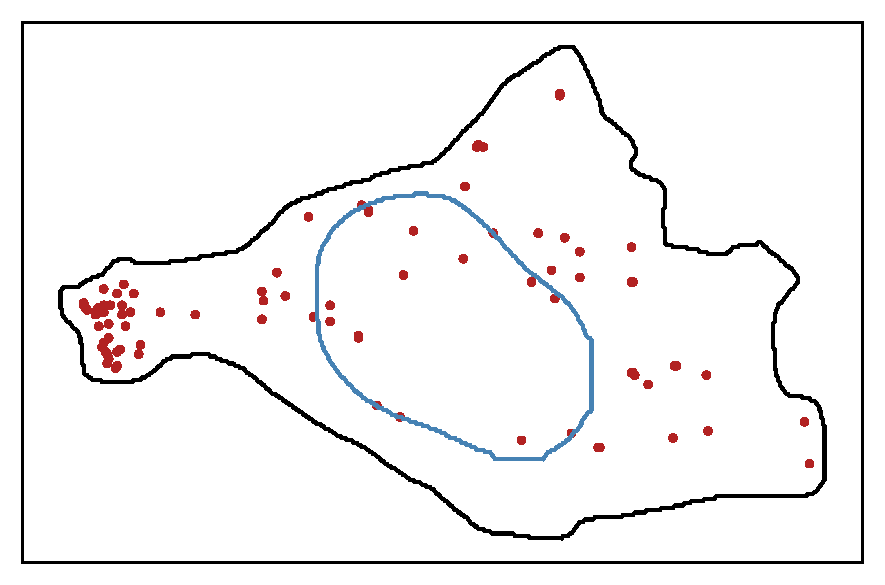
\includegraphics[trim={0.5cm 0.5cm 0.5cm 0.5cm},clip,width=\linewidth]{figures/chapter5/plot_protrusion}
		\subcaption{Protrusion}
	\endminipage
	\caption[RNA localization patterns]{RNA localization patterns from~\cite{CHOUAIB_2020}.
	Coordinate representations with RNA spots (\textit{red}), cell membrane (\textit{black}) and nuclear membrane (\textit{blue}).
	Detection and segmentation results are extracted and visualized with \emph{bigfish}}
	\label{fig:localization_patterns_racha_features}
\end{figure}

I use these hand-crafted features to train several binary classifiers, one for each localization pattern we want to recognize.
Five specific localization patterns are defined - foci, intranuclear, nuclear edge, perinuclear, protrusion - and the random pattern is considered as a default one.
Figure~\ref{fig:localization_patterns_racha_features} illustrates an example of these patterns with a coordinate representation.

To train the classifiers, manual annotations are needed as a ground truth.
I generate panels with the cropped original image of the individual cells and their coordinate representations.
These panels are then manually tagged with the appropriate localization pattern.
The manual classification result has been independently checked by several trained microscopists.
Ultimately, I end up with 810 annotated cells.
Counts of the annotations are presented in Table~\ref{table:real_dataset_chapter5}.

\begin{wraptable}{L}{0.50\textwidth}
	\centering
	\begin{tabular}{| c | c |}
		\hline
		Pattern & \# of cells \\
		\hline
		Random & 372\\
		Foci & 198\\
		Intranuclear & 73\\
		Nuclear edge & 87\\
		Perinuclear & 64\\
		Protrusion & 83\\
		\hline
	\end{tabular}
	\caption[Count of annotated cells]{Annotated cells}
	\label{table:real_dataset_chapter5}
\end{wraptable}

One way to evaluate how relevant is the feature space is to investigate the distribution of the annotated cells within it.
To do so, I reduce the dimensionality with a \ac{t-SNE} transformation~\cite{vandermaaten_2008} in order to visualize the features point cloud.
From the multi-dimensional feature space, I obtain a 2D vector representation I can plot.
In term of setting, I initialize the \ac{t-SNE} with a PCA transformation first and use a perplexity value of 30.

I also define a supervised learning problem with the training of 5 independent binary Random Forest classifiers~\cite{breiman_random_2001}.
The choice to design the problem as several binary ones instead of one multi-class problem allows me to define the localization patterns as non mutually exclusives.
Indeed, an individual cell can display several patterns at the same time, like \ac{RNA} clusters (foci) localizing around the nuclear membrane (nuclear edge).
For each model, I build a training set including all the cells of one class and a subsampling of cells from others classes, such that the imbalance is 1:4 for the positive class.
This is a ''one vs.\ all'' training strategy.
Eventually, I exploit the \ac{OOB} error allowed by the random forest design.
In such manner, the model can ''be fit in one sequence, with cross-validation being performed along the way.''~\cite{hastie_elements_2009}.
Random forest is an ensemble model of tree classifiers.
Each tree is trained on a subsample of the observations and a subset of features.
This ensembling framework makes random forest quite robust to overfitting.
For every sample, an \ac{OOB} prediction can be computed using only the trees fitted without the sample.
I initialize the random forests with 100 trees, a maximal depth of 3 and a minimum number of samples per splitter node of 2.
During the training, for each split, I consider a subset of 10 features and entropy criterion.
In addition, input dataset is rescaled to have zero mean and unit variance.

\subsection{Results}
\label{subsec:results_general_pattern}

Thanks to their design or their normalization, the selected spatial features are mostly invariant to \ac{RNA} concentration.
They enable the use of unsupervised or supervised methods to classify cells among several localization patterns.

\subsubsection{Unsupervised visualization}

\begin{figure}[]
    \centering
    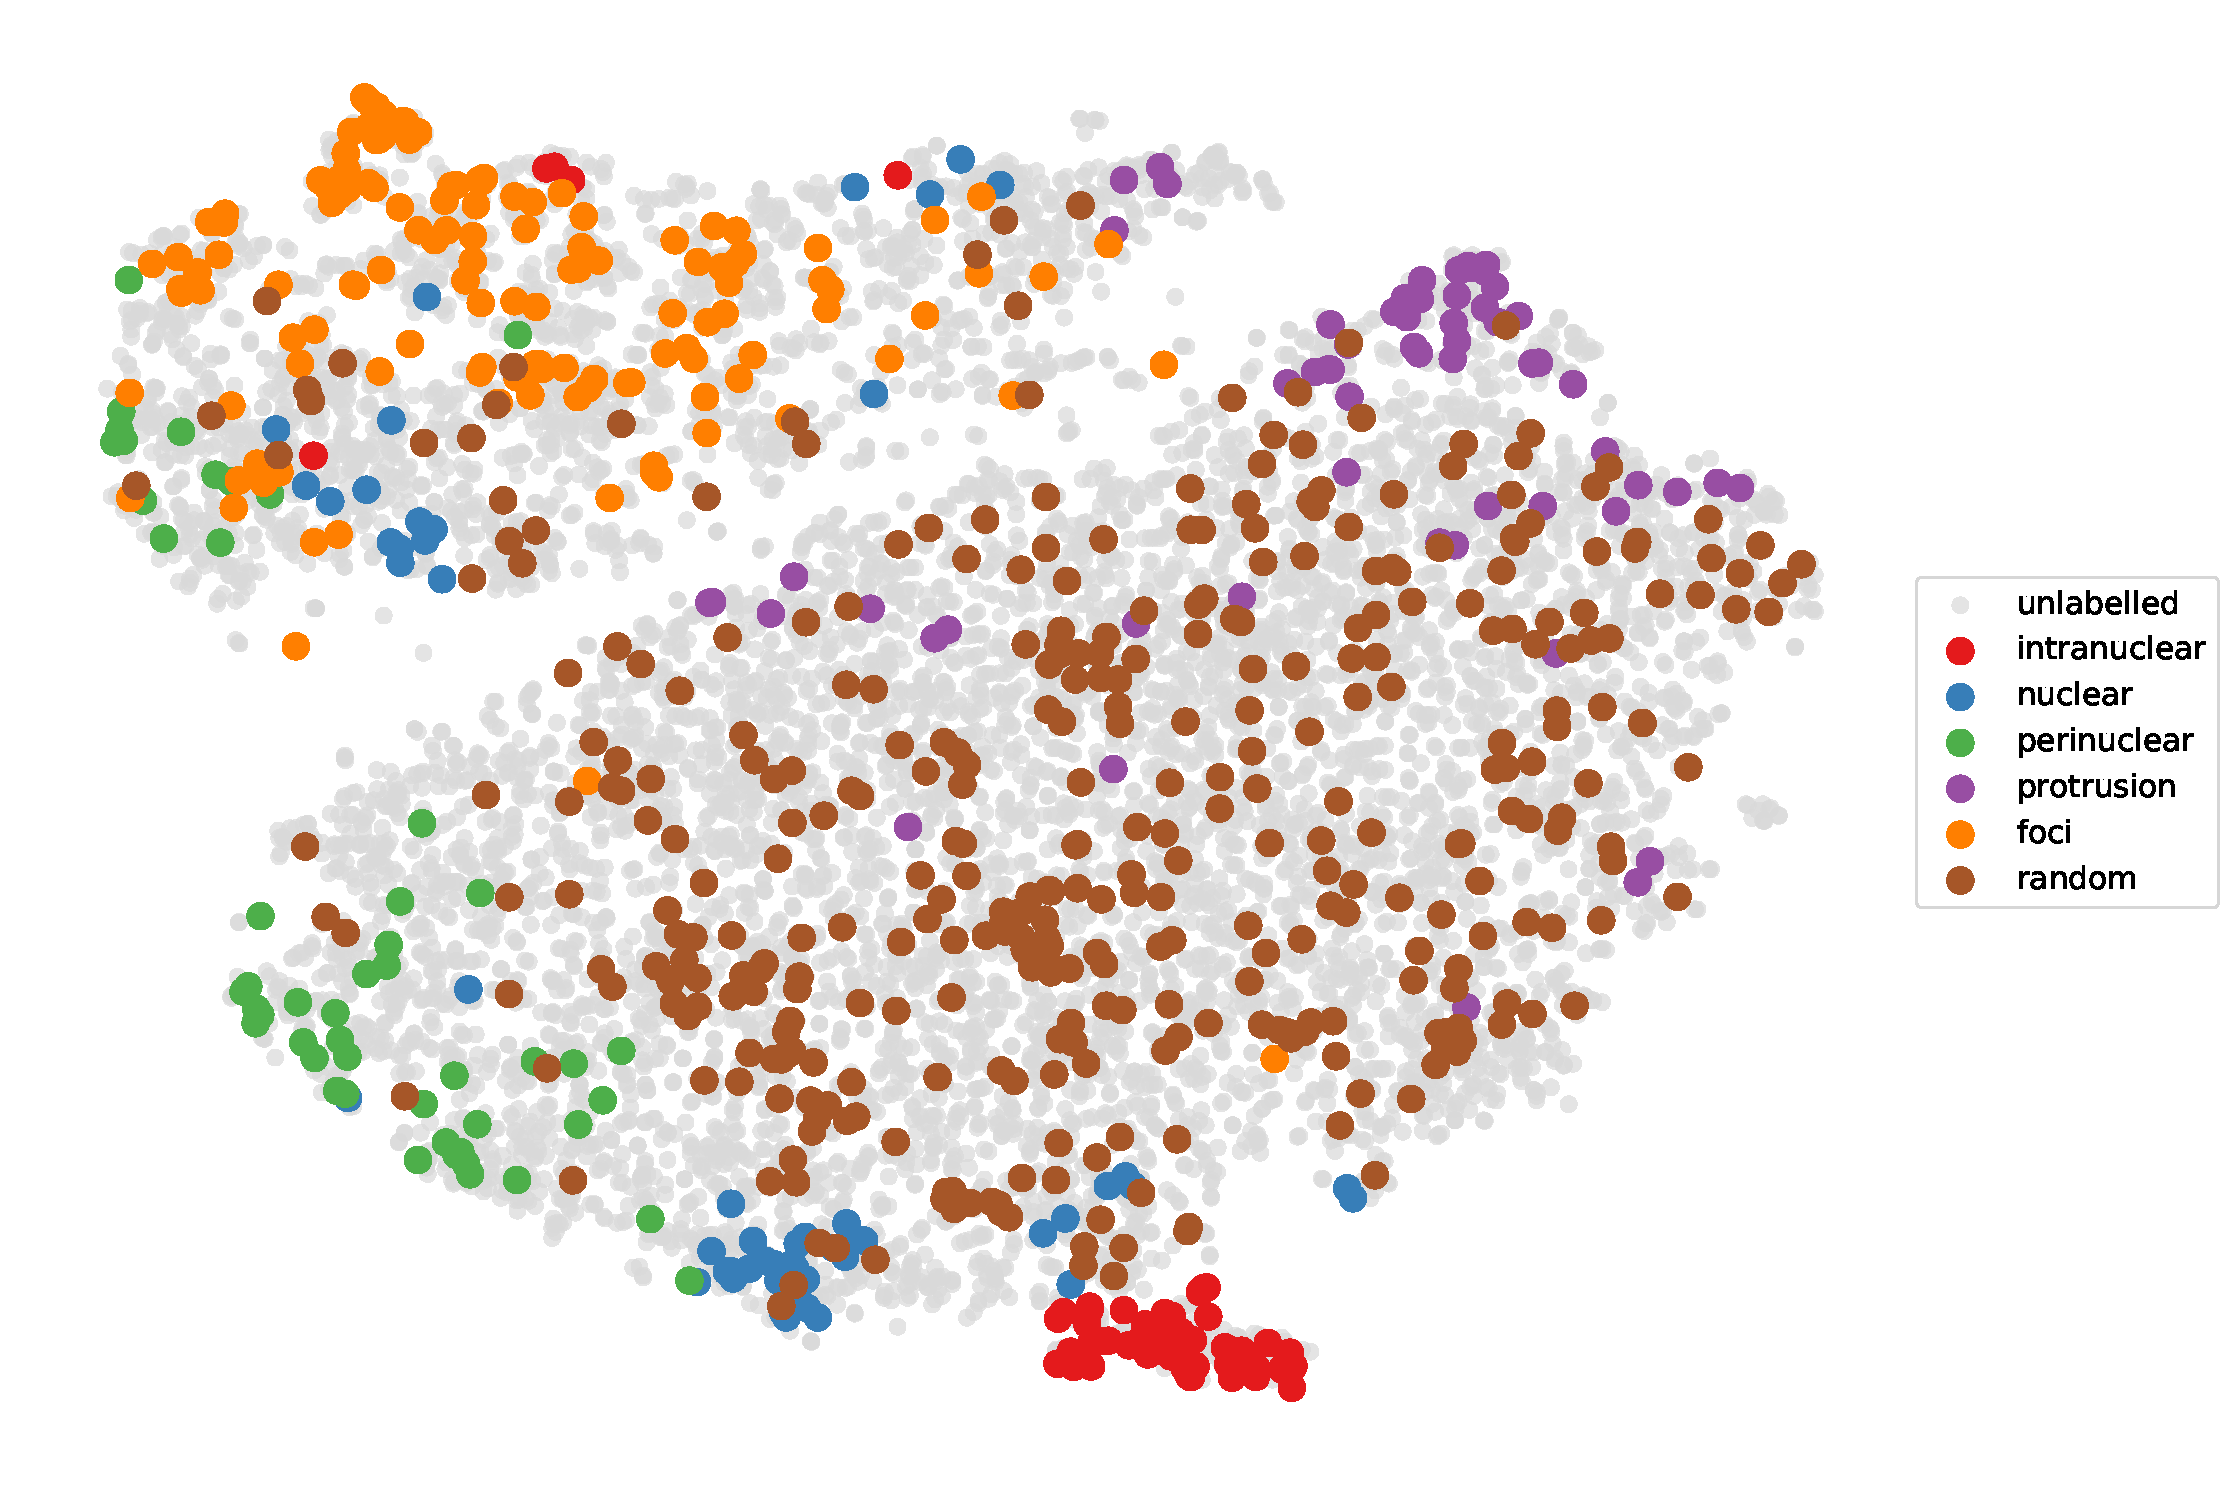
\includegraphics[width=\textwidth]{figures/chapter5/tsne_annotation_legend}
    \caption[t-SNE embedding of experimental cells]{t-SNE embedding from~\cite{CHOUAIB_2020}.
	Each point is a cell in the feature space after a t-SNE transformation.
	Manually annotated cells are colored according to their localization pattern.
	Cells that were not annotated or that had multiple patterns are colored in gray}
    \label{fig:tsne_annotation_racha}
\end{figure}

The resulting embedding from the \ac{t-SNE} algorithm can be observed in Figure~\ref{fig:tsne_annotation_racha}.
Cells with different patterns are localized in different regions of the embedded feature space.
Moreover, cells with the same annotations cluster in the same regions whether they correspond to the same gene or not.
With these observations it seems the hand-crafted features capture key information of the localization patterns and summarize well the manual annotations.

Initialized with a PCA transformation, a \ac{t-SNE} algorithm better preserves the global structure, thus enabling more relevant global interpretation.
In particular, we can discriminate at the top a large cluster of cells with a potential foci pattern from the rest of the cell population.
The resulting embedding also seems to polarize between nucleus-related patterns (bottom left) and the cell-related patterns (top right).
This polarization remains even among the subpopulation with potential foci pattern.
Such conclusion validates the design to let a cell being classified with several non-exclusive localization patterns.
Indeed, a foci can be localized in a relevant subcellular compartment.

\subsubsection{Gene aggregated classifications}

Not surprisingly, a feature space that discriminates well between classes also performs well when fed into a robust random forest classifier.
The \ac{OOB} accuracy score obtained for the different patterns is between 0.93 and 0.99, while a dummy classifier would return a 0.8 accuracy score (the dataset is built with 20\% positive samples).
The intranuclear pattern is the easiest to recognize.
In fact, it could be predicted by just thresholding the proportion of \ac{RNA} inside nucleus (almost all intranuclear cells have more than 80\% of their\ac{RNA}s that localize inside the nucleus).
On the opposite, the nuclear edge and perinuclear patterns are the most difficult to classify due to possible confusion with a random pattern or the lack of annotated cells.

\begin{wraptable}{R}{0.50\textwidth}
	\centering
	\begin{tabular}{| c | c |}
		\hline
		Pattern & Accuracy score\\
		\hline
		Random & -\\
		Foci & 0.95\\
		Intranuclear & 0.99\\
		Nuclear edge & 0.93\\
		Perinuclear & 0.93\\
		Protrusion & 0.94\\
		\hline
		\textit{Dummy classifier} & \textit{0.80}\\
		\hline
	\end{tabular}
	\caption[Random forest accuracy]{Random forest accuracy (OOB)}
	\label{table:accuracy_oob}
\end{wraptable}

For each cell, I can compute 5 binary predictions, one per pattern.
Individual cell is assigned to a pattern if the probability given by the random forest classifier for that pattern is higher than 0.5.
If no pattern is detected, cell is classified with a random localization pattern.
In total, I analyze 27 different genes through a population of 9,710 cells, with only one kind of transcript being targeted per cell.
The number of cells identified per gene varies, thus predictions are aggregated at the gene level.
This aggregation also facilitates the validation of biological insights and helps understanding the mechanism at stake for specific group of genes.
For every gene, I compute the proportion of cells displaying each indicated localization pattern.
Results are eventually reported in a heat map~\ref{fig:heatmap_racha}, for every gene and pattern.
Importantly, row values does not sum to one because classifiers (and so columns predictions) are independent.

\begin{figure}[]
    \centering
    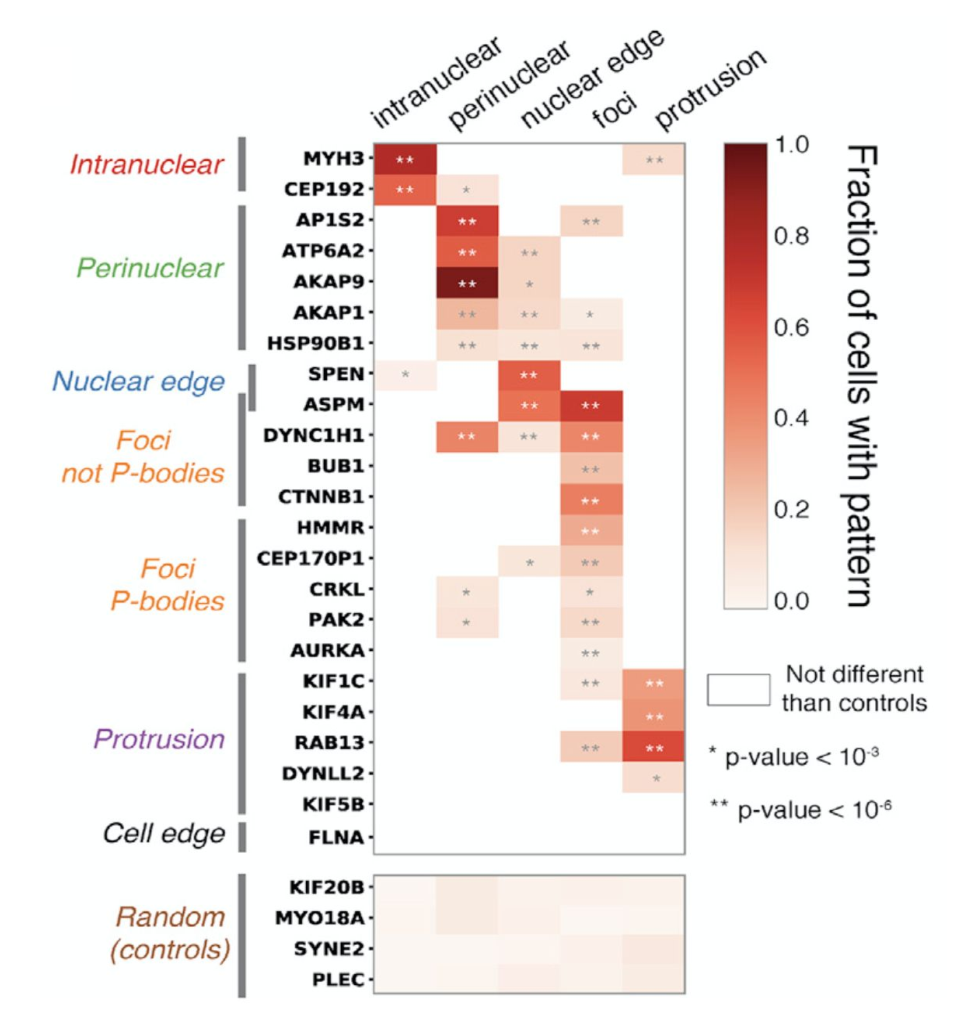
\includegraphics[width=\textwidth]{figures/chapter5/heatmap_racha_2}
    \caption[Heat maps with localization pattern classification results]{Heat maps from~\cite{CHOUAIB_2020} with the fraction of cells classified in the indicated pattern.
	(\textit{Top heat map}) Genes whose RNAs shows a localization preference.
	Only values significantly different from negative controls are colored (p-value computed with Fisher's exact test).
	(\textit{Bottom heat map}) Negative control with genes whose RNAs localize randomly.
	(\textit{Left bars}) Manual annotations of the genes are indicated with the same color scheme than Figure~\ref{fig:tsne_annotation_racha}}
    \label{fig:heatmap_racha}
\end{figure}

We manually identify a group of random genes that can be used as a control group: KIF20B, MYO18A, SYNE2 and PLEC.
Therefore, it is possible to perform statistical testing over the aggregated predictions.
A Fisher's exact test can measure if the proportion of cells observed with a pattern is significantly greater than the proportion observed in the control group (with a $\text{p-value} < 10^{-3}$).
Genes whose transcripts present a significant localization preference are reported in Figure~\ref{fig:heatmap_racha}.

Overall, we observe consistent results with the manual annotations performed by the biologists (the colored annotations in the \ac{t-SNE} plot~\ref{fig:tsne_annotation_racha} and the vertical colored bars next to the heat map~\ref{fig:heatmap_racha}).
The agreement between automated and manual classification holds with a high degree of statistical significance, except for FLNA and KIF5B.
FLNA transcripts are manually identified with a potential cell edge pattern.
However, such localization is difficult to recognize with the quantitative pipeline, mostly because the pattern is visible in 3D while my cell segmentation, and the spatial features resulting from it, is in 2D.
For these reasons we do not study in depth this localization pattern.

\subsubsection{Recognition of five localization patterns}

Apart from KIF5B, others transcripts localizing in cytoplasmic extensions (or protrusions) are correctly identified: KIF1C, KIF4A, RAB13 and DYNLL2.
The frequency of this pattern varies a lot, between 14\% and 62\% of cells classified, respectively for DYNLL2 and RAB13.
Interestingly, this pattern concerns four \ac{RNA}s encoding motor proteins: the three kinesins KIF1C, KIF4A, KIF5B and DYNLL2.

MYH3, another transcript encoding motor protein, localizes partially in protrusions, although it is not its most frequent localization pattern.
Most of the time, MYH3 transcripts remain in the nucleus, exhibiting an intranuclear pattern.
This is the most easily recognizable pattern: more than 55\% of cells spotting MYH3 and CEP192 \ac{RNA}s show an accumulation of transcripts inside nucleus.

The two genes observed with a nuclear edge pattern, ASPM and SPEN, have 50\% and 55\% of cells identified with this localization, respectively.

Several genes are identified with \ac{RNA}s in the perinuclear area: AKAP1, AKAP9, AP1S2, ATP6A2, and HSP90B1.
They ranged from 13\% (HSP90B1) to 93\% (AKAP9) of cells classify with said pattern.
Even with a small number of cells, HSP90B1 shows a significant perinuclear pattern compared to the control group.
Such observation is consistent with previous biological information about this gene: it contains a signal peptide that leads the translation (and the subsequent protein) on the endoplasmic reticulum, resulting in a perinuclear pattern through a 2D \ac{smFISH} experiment.
This also suggests that HSP90B1 transcript co-localizes with its protein.

A large number of transcripts exhibit a cluster-like localization pattern we call foci.
We classify them in two groups that we detail in the next Section~\ref{sec:translation_factories}.
The first group gathers transcripts accumulating in \ac{P-bodies}: AURKA, HMMR, CEP170P1, CRKL and PAK2.
The second group includes ASPM, DYNC1H1, BUB1 and CTNNB1 transcripts, accumulating in non-\ac{P-bodies} clusters we call translation factories.
It is noteworthy to mention that a number of genes exhibits foci with another localization preference in parallel like ASPM (nuclear edge), DYNC1H1, AP1S2, AKAP1, HSP90B1 (perinuclear), KIF1C and RAB13 (protrusion).
In general, non-\ac{P-bodies} genes have a higher proportion of cells classified with a foci pattern: between 24\% (BUB1) and 69\% (ASPM) cells while \ac{P-bodies} genes have between 7\% (AURKA) and 31\% (HMMR) cells.
Likewise, in term of molecule concentration, non-\ac{P-bodies} genes present a higher proportion of \ac{mRNA} in foci, varying from 9\% (BUB1) to 28\% (CTNNB1), while \ac{P-bodies} accumulate between 2\% to 15\% of \ac{mRNA}s.
This foci quantification is in line with the previously reported estimations in the literature of 10\% to 20\% \ac{mRNA}s clustered in foci~\cite{Pillai_2005, Hubstenberger_2017}.

\subsubsection{Cell-to-cell variability}

If we focus on the individual cell instead of the gene, \ac{RNA} localization appears highly variable.
For example, with CTNNB1 transcripts, there is either no foci at all or more than 60\% of \ac{mRNA}s clustered, depending of the cell observed.
For a better quantification of this intercellular variability, additional figures are presented in Appendix~\ref{ch:cell_pattern_classification}.
Cells of specific genes are plotted on \ac{t-SNE}~\ref{fig:tsne_proba_gene} and single cell results are summarized in heat maps~\ref{fig:heatmap_racha_cells}.
Pattern probabilities returned by classification models vary from cell to cell.
For a given gene, cells are dispersed on the \ac{t-SNE} plot, although a majority of them still accumulate in the expected area.
Finally, some cells have several localization patterns simultaneously.
As listed before, it the case for the cells with localized \ac{RNA} clusters, combining a foci pattern with a protrusion or a nucleus-related pattern.
Likewise, MYH3 cells frequently show an intranuclear and protrusion pattern.

In conclusion, my quantitative pipeline corroborates the manual observations and measures a high degree of heterogeneity of \ac{RNA} localization across different cells.
This variability is a general phenomenon, at least for HeLa cells, since it is seen with nearly all the genes analyzed in~\cite{CHOUAIB_2020}.
In comparison, \ac{RNA} localization in embryos appears to be much more stereotyped.

\section{The case for translation factories}
\label{sec:translation_factories}

Beyond the generic pattern recognition pipeline I have implemented, another important quantitative result concerns the characterization of a cluster-like localization pattern we name \emph{translation factory}.
This analysis is part of a broader investigation about the co-localization of \ac{mRNA}s and their encoded proteins, a major contribution of~\cite{CHOUAIB_2020}

\subsection{Introduction}
\label{subsec:introduction_translation_factories}

Studies previously mentioned focus on \ac{RNA} localization, but do not detect translated proteins~\cite{lecuyer_global_2007, battich_image-based_2013, Chen_2015, eng_seqfish_2019, Xia_2019}.
This makes impossible a complete analysis of the local translation mechanisms and their functions.
In~\cite{CHOUAIB_2020}, we performed a high-content screen in HeLa cells and visualize simultaneously the \ac{mRNA} and its encoded protein.
More precisely, we exploit a library of HeLa cell lines with a \ac{BAC} including a \ac{GFP}-tagged gene~\cite{poser_bac_2008} in order to visualize the selected proteins.
In parallel, and without compromising the localization of the \ac{mRNA}, the tag can be targeted with a \ac{smFISH} probe, allowing us to spot the \ac{mRNA} molecules.

Along with \ac{RNA} localization patterns, we observe occurrences of local translation in several subcellular areas.
For example, the phenomenon is observed in the nuclear membrane with the ASPM and SPEN transcripts.
Some local translations are expected, like HSP90B1 (an endoplasmic reticulum protein), ATP6A2 (in endolysosomes) or AKAP1 (an \ac{RBP} at the surface of mitochondria).
Others are discoveries like AKAP9 or AP1S2, whose \ac{mRNA}s are known to localized respectively in the Golgi or on endosomes.

Previous studies have exploited SunTag to visualize single molecules of nascent proteins~\cite{pichon_visualization_2016, Pichon_2018, Wu_2016}.
Here, this technique allows us to confirm that both ASPM \ac{mRNA}s and nascent proteins localized in nuclear membrane, thus suggesting a local translation.

The rest of this section goes a bit further by focusing on a translation-dependent foci pattern that differs from the more common \ac{P-bodies}.
We find four transcripts that accumulate in clusters, but do not colocalized with \ac{P-bodies} markers: BUB1, DYNC1H1, CTNNB1 and ASPM.
We name such complex \emph{translation factory}, where specific \ac{mRNA}s accumulate to be translated, and not repressed.
Indeed, we observe in these clusters a co-concentration of \ac{RNA} with nascent proteins, like in Figure~\ref{fig:translation_factory}.
Finally, my second contribution to~\cite{CHOUAIB_2020} consists in quantify this unexpected phenomenon, exploiting my cluster detections methods and experiments with a translation inhibition protocol.

\begin{figure}[]
    \centering
    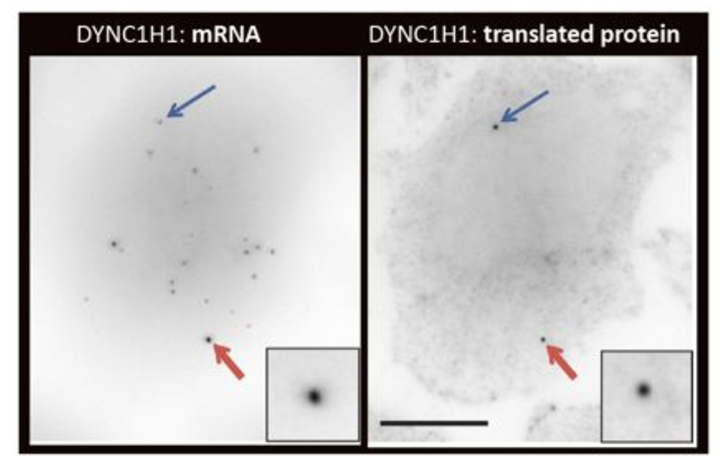
\includegraphics[width=\textwidth]{figures/chapter5/translation_factory}
    \caption[smFISH and SunTag images of DYNC1H1]{Colocalization between the DYNC1H1 transcript and its nascent protein, from~\cite{pichon_visualization_2016}.
	Transcripts and proteins are targeted with smFISH probes (\textit{Left}) and SunTag (\textit{Right}) respectively.
	\textit{Scale bar} is 10$\mu$m}
    \label{fig:translation_factory}
\end{figure}

\subsection{Materials and methods}
\label{subsec:materials_translation_factories}

In the continuation of the work presented in Section~\ref{sec:general_pattern_recognition}, the quantification is developed in Python and available online\footnote{\url{https://github.com/Henley13/paper_translation_factories_2020}}.

\subsubsection{Translation inhibition}

To analyze the role of translation in the \ac{mRNA} localization we perform several mirror experiments where translation is inhibited.
For this task we use puromycin or cycloheximide drugs.
The former inhibits translation by releasing the nascent peptide chain from the ribosomes.
On the opposite, the later inhibits translation by freezing the ribosomes on the \ac{mRNA}s.
The fact that such treatments would alter the localization pattern is an evidence that it's a translation driven mechanism.
Furthermore, by composing with these two treatments, we can clarify if a translation-dependent localization requires the whole protein translation or just its nascent peptide chain.
In the case of ASPM gene, we observe for example that the localization patterns (nuclear edge and foci) disappear with puromycin, but not with cycloheximide.
It suggests that the \ac{mRNA} localization requires the nascent protein.

For a quantification purpose we develop a \ac{smiFISH} screen to compare untreated cells and cells treated with puromycin for 10mn.
Coupled with my computational pipeline, I can measure the impact of a translation inhibition.

\subsubsection{Cluster detection}

Both on the treated and untreated cells I re-apply my spot detection algorithms, the decomposition of dense areas with large agglomeration of spots and ultimately the detection of \ac{RNA} clusters, directly from their detected coordinates (see Subsection~\ref{subsec:materials_general_pattern}).
It is important to note that the cluster detection is distinct from the dense area decomposition.
Such areas can indeed be processed in a way that no cluster is detected afterward.

\subsection{Results}
\label{subsec:results_translation_factories}

\subsubsection{Translation-dependent localization}

\begin{figure}[]
    \centering
    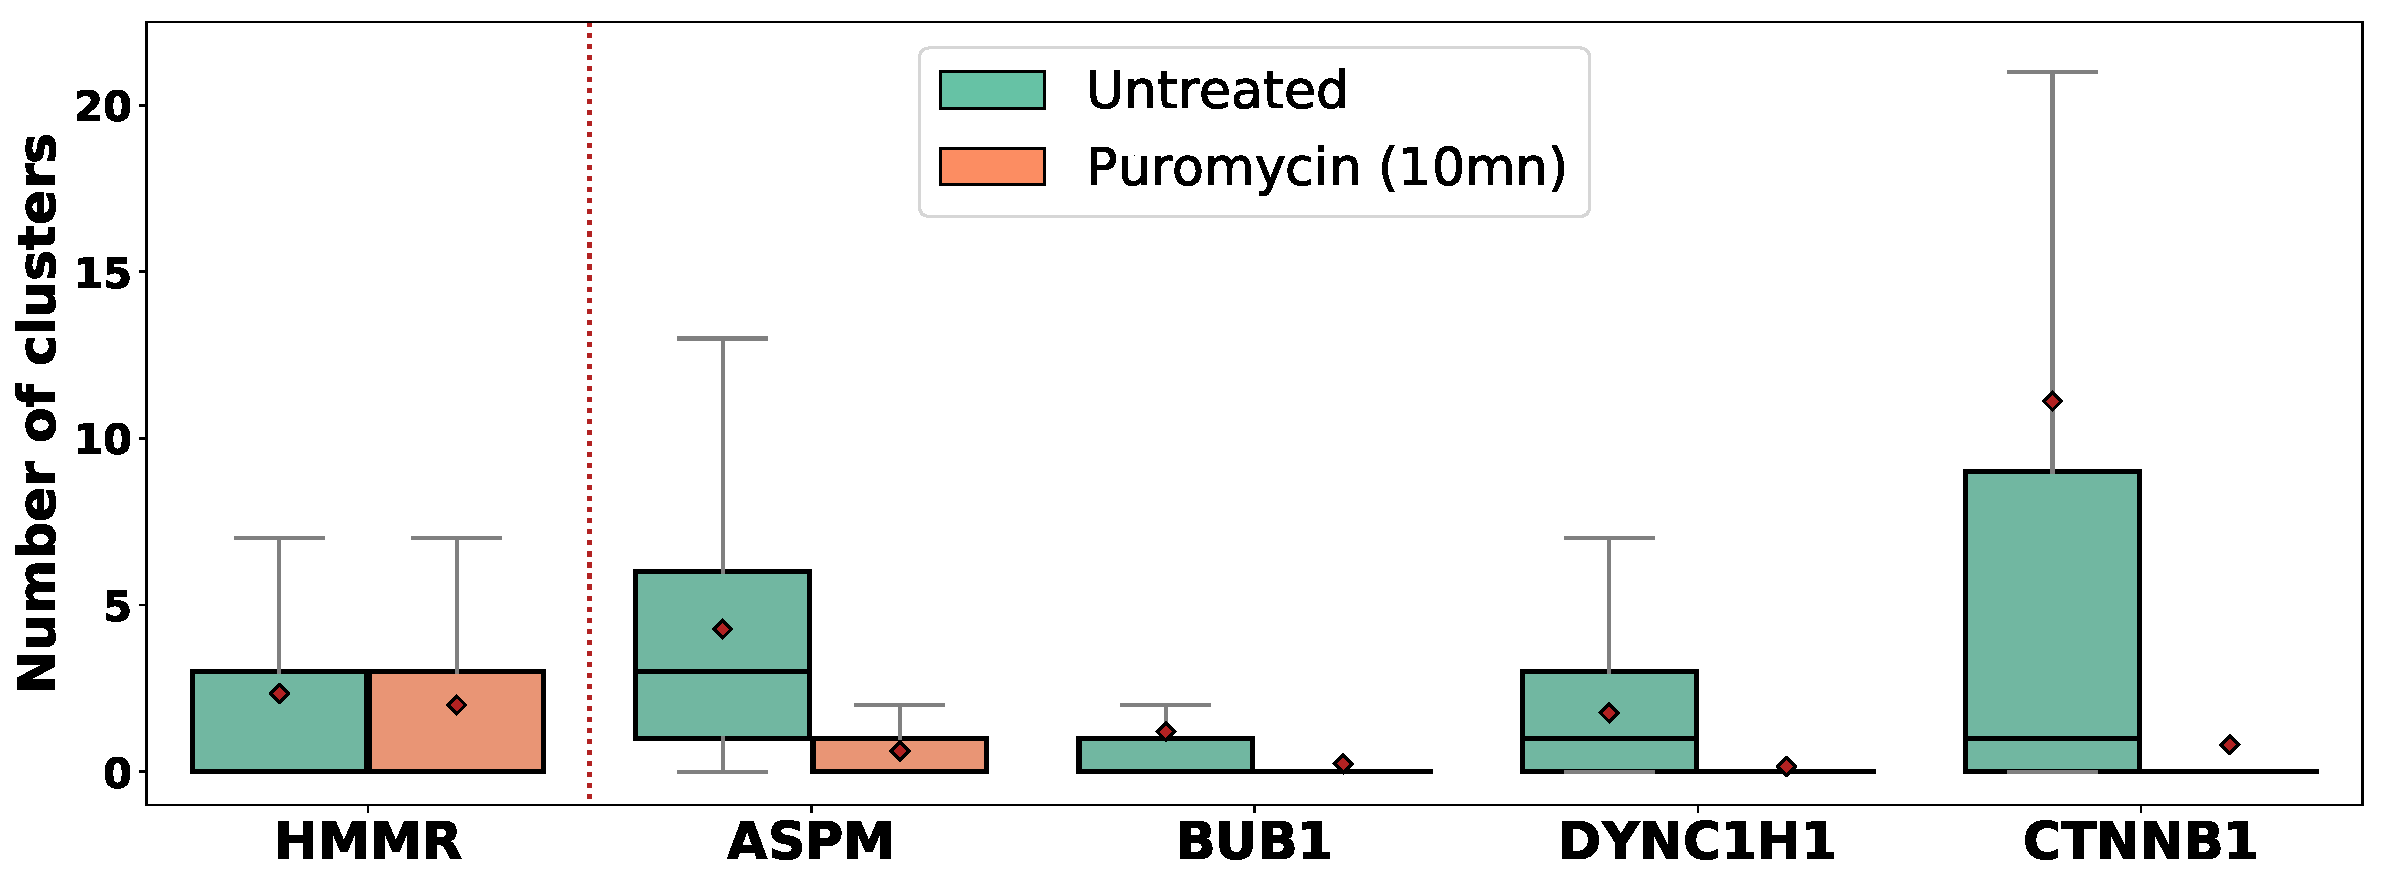
\includegraphics[width=\textwidth]{figures/chapter5/plot_puromycin}
    \caption[Box plot with the number of detected RNA clusters]{Box plot with the number of detected RNA clusters for different genes and treatments.
	Red diamonds are the mean and the \textit{whiskers} equal 1.5 the interquartile range}
    \label{fig:plot_puromycin}
\end{figure}

An obvious indicator to assess if a foci pattern is disrupted is the number of \ac{RNA} clusters detected per cell.
When I compare treated and untreated cells, the difference is clear for the four genes BUB1, DYNC1H1, CTNNB1 and ASPM.
Their transcripts usually accumulate in foci, but with the presence of puromycin drug, \ac{mRNA}s are dispersed within the cell and the number of detected clusters drops.
This is what we call translation factories: noteworthy cluster-like complexes where specific \ac{mRNA}s are translated.

As a comparison, in Figure~\ref{fig:plot_puromycin}, I perform the same analysis with HMMR, a gene classified as \ac{P-bodies}.
The difference is striking, as the foci pattern seems unchanged when early translational termination happens.
In addition, a dual-color \ac{smiFISH} allows us to visualize two different transcripts at the same time and thus to confirm that the foci detected with the four translation factories genes are not overlapping.
These are distinct and specialized \ac{RNA} complexes.

An analysis with a finer granularity is detailed in Appendix~\ref{ch:cell_pattern_classification} and especially in Figure~\ref{fig:tsne_proba_gene}.
For a same gene like DYNC1H1 the impact of inhibited translation (by puromycin) can be observed cell-to-cell.
Treated cells are much more dispersed in the \ac{t-SNE} plot.

\subsubsection{CTNNB1 factories}

Among the four genes with translation factories, cytoplasmic clusters of CTNNB1 \ac{mRNA} present a surprising regulation mechanism.
This \ac{mRNA} encodes the $\beta$-catenin protein, which is the main transcription factor of the Wnt signaling pathway~\cite{Grainger_2018}.
The later is notably known to play a role in carcinogenesis and embryogenesis.
The Wnt signal allows the $\beta$-catenin protein to translocate and accumulate in the nucleus in order to activate targeted transcriptions.

The existence of translation factories offers a new insight on the dynamic at stakes in the presence of Wnt.
$\beta$-catenin is degraded in a ''destruction complex'' that involves APC, AXIN, in addition to the kinases CK1$\alpha$ and GSK3~\cite{stamos_catenin_2013}.
When the Wnt pathway is activated, these molecules are recruited to the cell membrane and can no longer interact with $\beta$-catenin, thus stopping its degradation.
As a consequence, we observe that $\beta$-catenin is highly expressed and accumulates in the nucleus.
Interestingly, in the presence of Wnt, we also observe that the CTNNB1 \ac{mRNA} foci disappear.
This phenomenon suggests a relation between the degradation of $\beta$-catenin and the foci formation.
In~\cite{CHOUAIB_2020} we demonstrate that CTNNB1 translation factories rely on the nascent peptide chain, but it seems they also require the ''destruction complex''.
When the different components of this complex are disrupted, the \ac{mRNA} clusters tend to disappear.
Moreover, these components accumulate in the foci.
CTNNB1 translation factories are altogether sites of both $\beta$-catenin synthesis and degradation.
As~\cite{Chin_2020} summarizes it, these factories are ''sites of co-translational protein degradation, where CTNNB1 protein rapidly comes into contact with the destruction complex, offering an elegant mechanism to tightly control the cellular levels of potent signaling pathway effectors''.

\section{A translation and cell cycle dependent centrosomal pattern}
\label{sec:centrosomal}

In~\cite{safieddine_choreography_2021} the analysis pipeline is far more mature.
It benefits from the development of FISH-quant V2 and the improvements published in the literature about cell segmentation.
My contribution consists in quantifying the centrosomal localization pattern observed for some \ac{mRNA}s.

\subsection{Introduction}
\label{subsec:introduction_centrosomal}

We keep exploring specific \ac{RNA} localization patterns and local translation in~\cite{safieddine_choreography_2021}.
The paper focuses on transcripts localizing at the centrosomes.
They are the \ac{MTOC} in most animal cells and are composed of two centrioles surrounded with a \ac{PCM} - a highly structured mass of proteins.
These organelles are a heritage from ancient eukaryotic cells.
Plants, fungi (and some species of flatworm and flies) use a different mechanism to structure their microtubules.

Centrosomes have an important role in cell division, in addition to regulate cell motility and polarity~\cite{wu_2017}.
Concerning cell division, centriole duplication ensures that each daughter cell inherits two centrioles after mitosis.
In G1 phase, there is one centrosome per cell, with two centrioles connected by a linker.
During S phase, nucleation of the procentrioles (the daughter centrioles) happens.
By G2 phase, these procentrioles elongate.
After the two centrioles pairs mature and the \ac{PCM} expands, the two centrosomes are separated during the G2-M transition.

First observations of a \ac{mRNA} accumulation at the centrosomes are made on Xenopus early embryos~\cite{Groisman_2000}, with cyclin B1 \ac{mRNA}s concentrating at the mitotic apparatus.
Subsequent approaches of microscopy with \ac{FISH} techniques allow to image \ac{mRNA} localization in Drosophila~\cite{lecuyer_global_2007, wilk_diverse_2016} and human cell lines~\cite{Sepulveda_2018, CHOUAIB_2020}.
As these \ac{mRNA}s encode for known centrosomal proteins, these studies suggest a phenomenon of local translation.

In~\cite{safieddine_choreography_2021}, we identify 8 \ac{mRNA}s with a centrosomal pattern.
Remarkably, these \ac{mRNA}s combine both spatial and temporal distribution patterns.
Their localization appear to be translation dependent, through the synthesis of a nascent protein, and cell cycle dependent.
Moreover, these \ac{mRNA}s conserved their properties in both human and drosophila cell lines.

\subsection{Materials and methods}
\label{subsec:materials_centrosomal}

The quantitative analysis presented here exploits an improved version of \emph{bigfish}, especially for the spot detection.
The main blocks that will be published in FISH-quant V2 are already present.
This work is developed in Python and the code repository is public\footnote{\url{https://github.com/Henley13/paper_centrosome_2020}}.

\subsubsection{Experimental data}

With an Opera Phenix High-Content Screening System (PerkinElmer) we acquire 3D images with around 35 z-slices and a spacing of 0.3$\mu$m.
In total, and after curation, we collect 3,678 \ac{FoV}s of HeLa cell line spotting 12 different transcripts, sometimes treated with translation inhibitors like puromycin or cycloheximide.
In addition to the \ac{smFISH}, each image includes three fluorescent labels to visualize the nucleus (DAPI), the cell (CellMask\textsuperscript{\texttrademark}) and the centrosomes (Centrin1-\ac{GFP}) as illustrated in Figure~\ref{fig:fov_adham}.

\begin{figure}[]
    \centering
    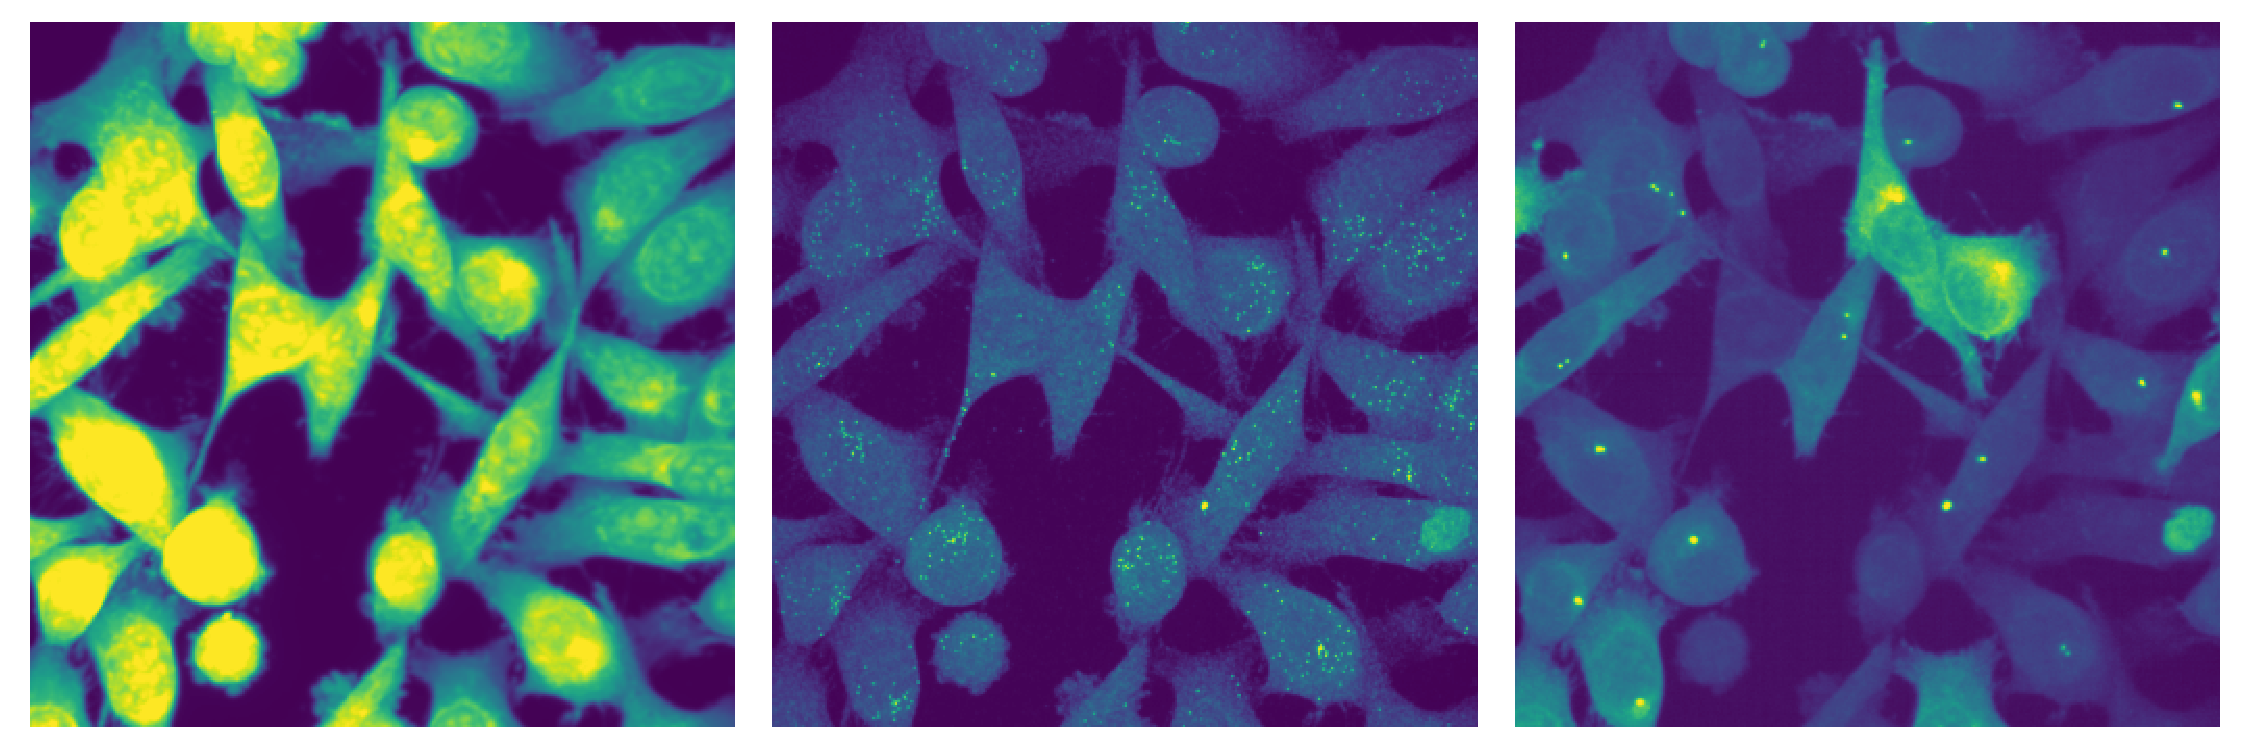
\includegraphics[width=\textwidth]{figures/chapter5/FoV_BICD2}
    \caption[Contrasted image with CellMask\textsuperscript{\texttrademark}, smFISH and GFP channels]{Contrasted image with CellMask\textsuperscript{\texttrademark} (\textit{left}), smFISH (\textit{center}) and GFP (\textit{right}) channels.
	Targeted transcript is BICD2.
	Images are projected in 2D.
	Plot built with \emph{bigfish}}
    \label{fig:fov_adham}
\end{figure}

\subsubsection{RNA and centrosome detection}

In~\cite{safieddine_choreography_2021}, and for the first time, I use the threshold-free spot detection described in Chapter~\ref{ch:chapter2}.
This heuristic helps me to scale the detection to thousands of images.
\ac{RNA} detection is followed by the decomposition of dense areas and the detection of \ac{RNA} clusters, everything being processed from the \ac{smFISH} channel projected in 2D (for the sake of simplicity).

The novelty in this paper is the detection of centrosomes from a \ac{GFP} channel (projected in 2D too).
Since the centrosome appears as a much larger spot than the individual \ac{RNA} molecule, I detect it like I would detect a \ac{RNA} cluster, but in the \ac{GFP} channel and with tuned parameters.
It works surprisingly well and enables me to scale the centrosome detection as well.
The final results can be observed in Figure~\ref{fig:centrosomes}.

\begin{figure}[]
    \centering
    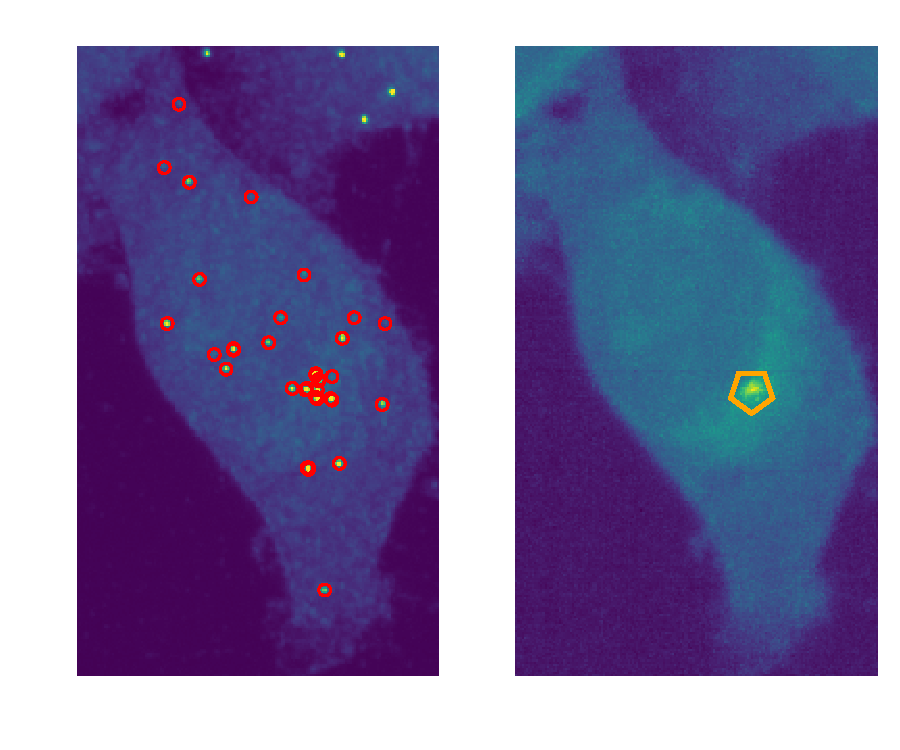
\includegraphics[width=\textwidth]{figures/chapter5/centrosomes}
    \caption[RNA and centrosome detection results]{Contrasted image with detected RNAs on a smFISH channel (\textit{left}) and detected centrosome on a GFP channel (\textit{right}).
	Targeted transcript is BICD2.
	Plot built with \emph{bigfish}}
    \label{fig:centrosomes}
\end{figure}

\subsubsection{Cell and nucleus segmentation}

Nucleus and cell segmentation is performed with a pretrained cellpose model~\cite{stringer_cellpose_2021}, respectively from the 2D DAPI and CellMask\textsuperscript{\texttrademark} channels.
It is based on a modified U-Net architecture~\cite{Ronneberger_unet} and trained on a dedicated and diversified dataset released by the authors.
The performance of a deep learning model like cellpose makes the segmentation step scalable with little or no manual intervention.
Here, I parametrize cellpose to segment nuclei with a diameter of 14.4$\mu$m and cells with a diameter of 22.7$\mu$m, in average.
It appears that cellpose is quite sensitive to the diameter set, a priori, as the model resizes the input image accordingly.
Ultimately, I check that every nucleus matches a segmented cell.
Isolated cells or isolated nuclei are removed.

Then, I extract and save the collected information for all individual cells.
Eventually, 54,263 individual cells are identified, with at least 10 detected \ac{RNA}s and 1 or 2 centrosomes.

\subsubsection{Centrosomal features and cell cycle classification}

I adapt the spatial features developed for~\cite{CHOUAIB_2020} to characterize a centrosomal \ac{RNA} pattern at the single-cell level.
In particular, I define the centrosomal region as a disk with 2000nm radius around the \ac{MTOC}.
This distance threshold is empirically set.
From there, I can compute any potential accumulation of \ac{RNA}s within centrosome's neighborhood, normalized by the expression level observed for each cell.
An example of such accumulation can be seen in Figure~\ref{fig:centrosomes}.
The detail of the different features implemented is described in Section~\ref{subsec:expert_features} and illustrated in Figure~\ref{fig:centrosome_features}.
All the features are based on the detection and segmentation results previously extracted.

In order to classify the cell cycle, we compute nucleus morphological features from the DAPI channel and the segmentation results using CellCognition~\cite{held_cellcognition_2010}.
Completed with manual annotations it allows us to discriminate interphase, early mitosis and late mitosis stages.

\subsection{Results}
\label{subsec:results_centrosomal}

\subsubsection{Centrosomal mRNAs}

\begin{figure}[]
    \centering
    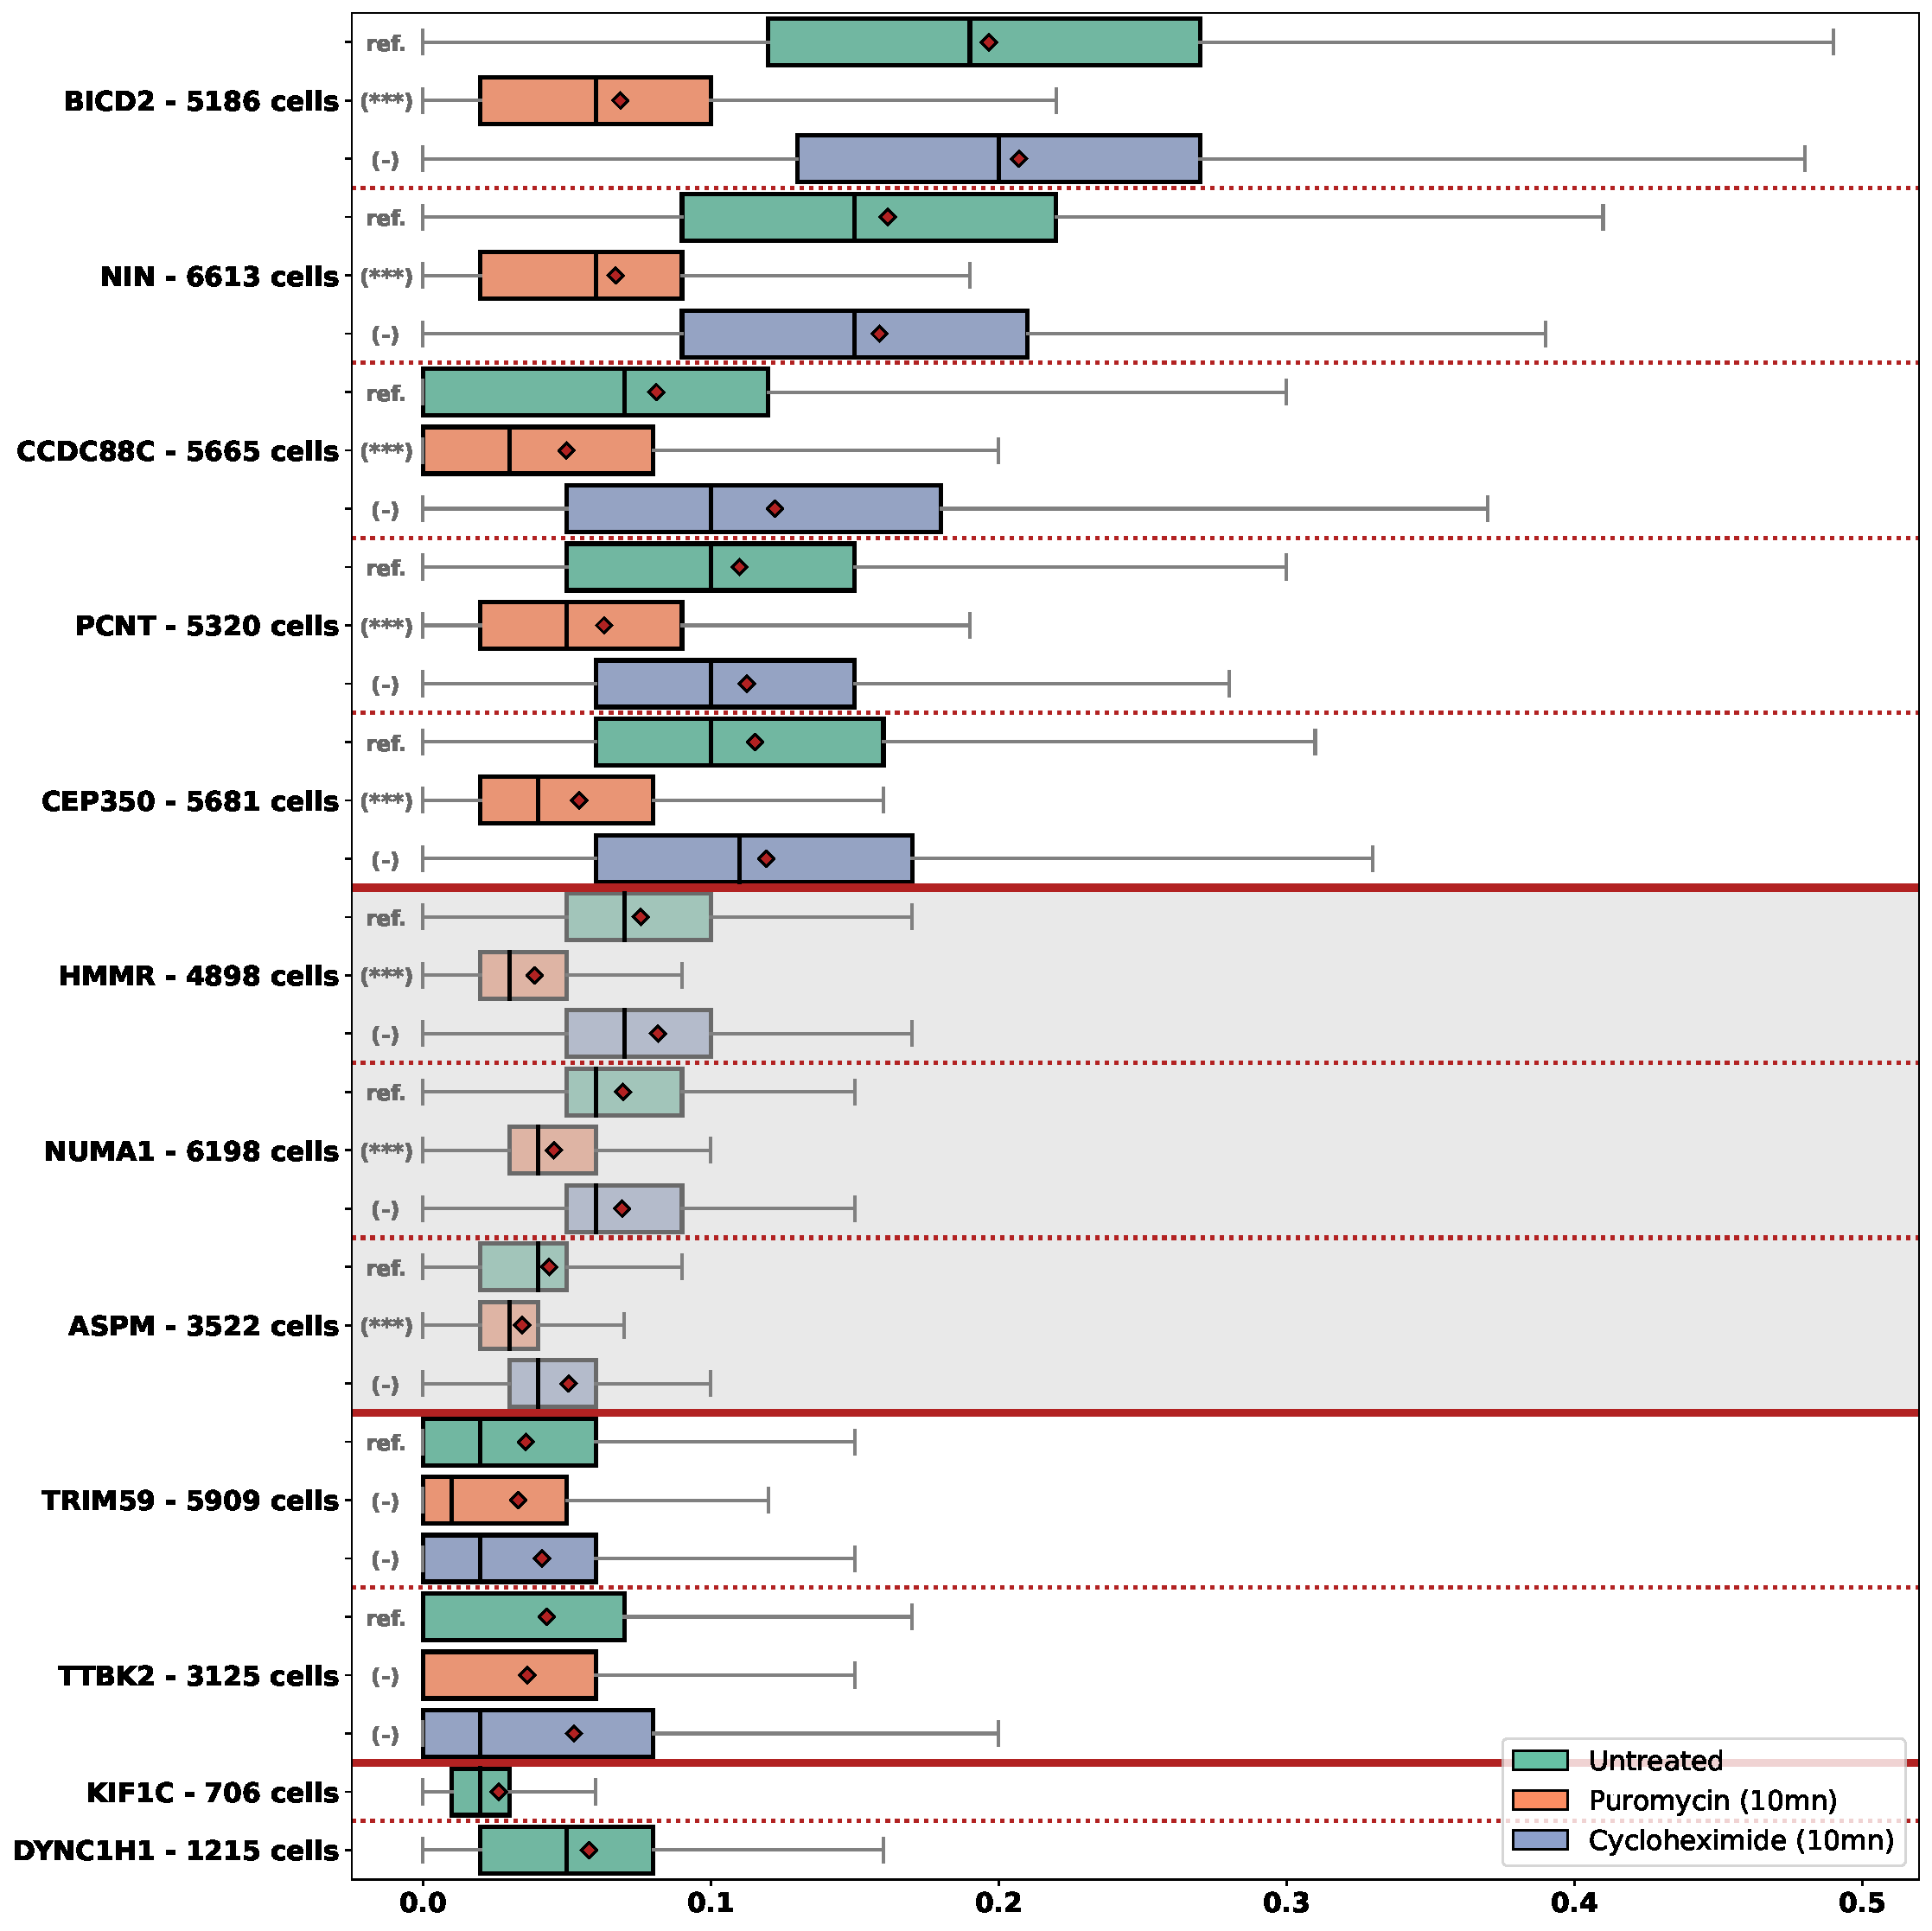
\includegraphics[width=\textwidth]{figures/chapter5/plot_rna_centrosome}
    \caption[Box plot with the proportion of centrosomal mRNAs]{Box plot with the proportion of centrosomal mRNAs in cells (interphase and mitotic phase), for different genes and treatments.
	Red diamonds are the mean and the \textit{whiskers} equal 1.5 the interquartile range.
	HMMR, NUMA1 and ASPM (in \textit{gray}) are endogenous mRNAs, the rest are BAC-transcribed mRNAs.
	TRIM59, TTBK2, KIF1C and DYNC1H1 are used as control mRNAs.
	A one-sided Welch’s t-test is used to evaluate significance (***: p-value < 0.001)}
    \label{fig:plot_rna_centrosome}
\end{figure}

My contribution in~\cite{safieddine_choreography_2021} is to quantify what biologists named and classify as centrosomal \ac{mRNA}s.
Among the centrosomal protein-coding genes analyzed, we find 8 human \ac{mRNA}s that accumulate in centrosome's neighborhood: BICD2, NIN, CCDC88C, PCNT, CEP350, HMMR, NUMA1 and ASPM.
I design a quantitative pipeline to process a high-content screening dataset and compute the proportion of \ac{mRNA}s detected around a centrosome.
The results are reported in Figure~\ref{fig:plot_rna_centrosome}.
In addition to the centrosomal transcripts, I also process control genes without the studied pattern, for comparison purpose.
While TRIM59 and TTBK2 present no specific localization pattern, KIF1C and DYNC1H1 are respectively and frequently identified with protrusion and foci patterns (among other localizations).

Two main observations can be drawn from this plot.
First, most of the centrosomal \ac{mRNA}s present a higher proportion of transcripts around the centrosomes: from 4.4\% (ASPM) to 19.7\% (BICD2), against 4.0\% for the control genes, in average.
The difference is less evident with ASPM transcripts, for example, with a lower proportion  of centrosomal \ac{mRNA}s than DYNC1H1 (5.8\% in average).
As a control, DYNC1H1 transcripts accumulate in clusters and localize within the nuclear region and thus can be easily confused with a centrosomal pattern.
This can illustrate a limitation of my quantification.
If the centrosomal pattern is too complex to be characterized with only one spatial feature, the use of several centrosomal features, coupled with a classification pipeline could be beneficial, like in~\cite{CHOUAIB_2020}.
In addition, performing the spot detection on 2D projected images instead of 3D stacks leads to a loss of information for the final quantitative results.
Second, we can observe the impact of a puromycin treatment, with a drop of centrosomal \ac{mRNA}s.
A long puromycin treatment can even prevent the mitosis.
On the opposite, with a cycloheximide treatment, the pattern remains unchanged for most of the targeted genes.
Similarly to the translation factories, it suggests that the centrosomal pattern is driven by the presence of nascent peptide chains.

By exploiting live cell imaging and tracking \ac{mRNA} molecules we further demonstrate that their localization implies an active polysome transport.
In particular, ASPM polysomes appear to move at speeds ranging from 0.5 to 1$\mu$m/s, a rate compatible with motor-driven transport.

\subsubsection{A cell cycle regulated localization}

Several iterations between manuel annotations and an automated classifier help to identify mitotic cells according to their mitosis phases, and thus refine and deepen our results.
Five \ac{mRNA}s exhibit a centrosomal localization pattern during interphase and early mitosis: HMMR, BICD2, CEP350, PCNT and NIN.
In addition, HMMR is the only gene whose \ac{mRNA}s and proteins co-localized at cytokinetic bridge in telophase.
Lastly, ASPM and NUMA1 localize only during mitosis and CCDC88C in interphase.
However, while NUMA1 \ac{mRNA}s localize during early mitosis (prophase and prometaphase), a centrosomal accumulation of ASPM \ac{mRNA}s can be observed for every mitotic phase.
All in all, these results reveal an elegant \emph{choreography} of \ac{mRNA} localization, cell cycle regulated and translation driven.

\section{The key role of KIF1C in protrusion pattern}
\label{sec:protrusion}

In~\cite{pichon_kinesin_2021} I benefit from a proven and mature pipeline to extract quantitative results from a \ac{smFISH} high content screening study.
My contribution consists in quantifying a protrusion pattern manifested by the accumulation of \ac{mRNA}s in cell extensions.

\subsection{KIF1C and protrusion mRNAs}
\label{subsec:introduction_protrusion}

Three main \ac{RNA} transport mechanisms are reported in the literature: a localized protection from \ac{RNA} degradation, a random diffusion coupled with a targeted entrapment and an active \ac{RNA} transport along the cytoskeleton, with specific motor proteins~\cite{Medioni_2012, Bovaird_2018}.
In this section, we focus on the active transport mechanism.
As an example, in vertebrates, the $\beta$-actin \ac{mRNA} has a \emph{zipcode} sequence that the \ac{RBP} ZBP1 will recognize, hence allowing the transport of the \ac{mRNA} molecule along microtubules and actin filaments~\cite{Oleynikov_2003}.

More specifically, we investigate the role of the kinesin KIF1C that accumulates in cell protrusion (see Figure~\ref{fig:heatmap_racha}) and encodes a microtubule motor protein.
This protein interacts with a specific group of \ac{mRNA}s defined as APC-dependent (they require the APC protein to localize~\cite{wang_extracellular_2017}).
KIF1C protein binds a subset of these \ac{mRNA}s and transports them to cell extensions where they exhibit cluster-like structures: NET1, TRAK2 and RAB13 .
Interestingly, this kinesin protein also actively transports its own transcript to protrusions.

Finally, we demonstrate that KIF1C is needed to transport these APC-dependent \ac{mRNA}s to protrusions along microtubules and to form their clusters.
Indeed, these foci are not observed in cell extensions when KIF1C motor is absent.
KIF1C seems to have a dual function as microtubule motor and ''\ac{mRNA} anchoring module promoting clustering''~\cite{pichon_kinesin_2021}.

\subsection{Quantification of peripheral mRNAs}
\label{subsec:materials_results_protrusion}

This study is an opportunity to exploit a proven FISH-quant V2 and to scale a quantitative analysis that characterizes protrusion \ac{RNA}s from HeLa cells.
I identify 27,644 individual cells, spotting \ac{mRNA}s from 40 different genes, including KIF1C, APC-dependent \ac{mRNA}s and control transcripts.
For every cell, I perform an automated spot detection, nucleus and cell segmentation, from 2D projected images.
I compute RDI Calculator features from~\cite{stueland_rdi_2019}, especially the peripheral distribution index that measures how close the \ac{RNA}s localize to the cell periphery (see Section~\ref{subsec:expert_features}).
The greater the value of the index, the more concentrated in the protrusion are the transcripts.

\begin{figure}[]
    \centering
    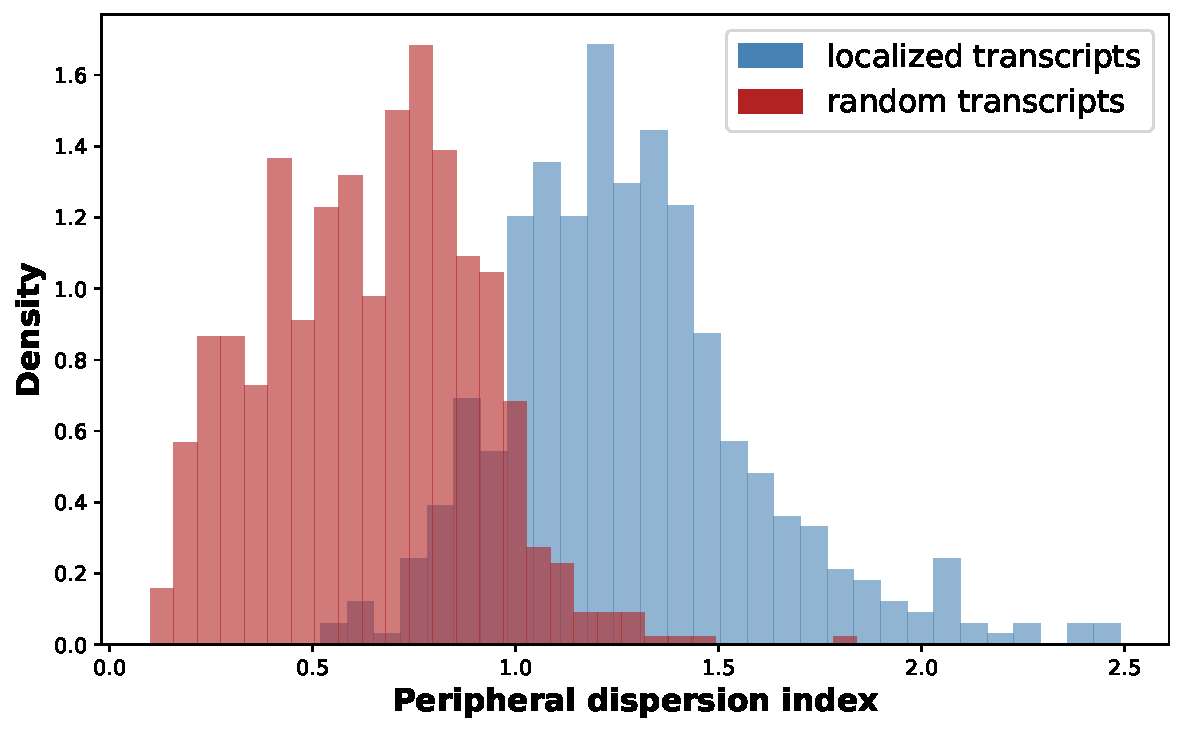
\includegraphics[width=\textwidth]{figures/chapter5/helacentrin_distribution_pdi}
    \caption[Histogram of the peripheral distribution index]{Histogram of the peripheral distribution index for two group of transcripts.
	Localized transcripts include: KIF1C, TRAK2 and NET1.
	Control transcripts include NEK9, NIN, NPM1, OBSL1, OLA1, PAX2, PKHD1, RGS14, SMAD7 and SPAST}
    \label{fig:xavier_pdi}
\end{figure}

In Figure~\ref{fig:xavier_pdi}, I compare two groups of transcripts: KIF1C, TRAK2 and NET1, three \ac{mRNA}s that bind to KIF1C protein for active transport to the protrusions, and a control group unrelated to KIF1C.
For the peripheral distribution index, a completely random distribution has a value of 1.
Here, as expected, the protrusion \ac{mRNA}s exhibit a biased spatial distribution toward the cell extensions.
Finally, RAB13 (that is not included in this analysis), KIF1C, TRAK2 and NET1 are the four transcripts that are enriched in cell protrusion and colocalized with their proteins.

\section{Conclusion}
\label{sec:conclusion_chapter5}

In this chapter, I present several applications of FISH-quant V2.
Based on high content screening, from HeLa cell lines, I perform large scale quantitative analyses to support different biological insights.
In total, several dozens of transcripts have been analyzed across 100,000 individual cells and hundreds of fluorescent bioimages.

In~\cite{CHOUAIB_2020}, I exhibit the high level of heterogeneity in term of \ac{mRNA}s localization, for a given cell population.
The classification pipeline designed enables the identification of complex localization patterns: intranuclear, nuclear edge, perinuclear, foci and protrusion.
The foci pattern itself is in fact composed of two different cluster-like structures of \ac{mRNA}s.
The first one repressed transcripts and store them in \ac{P-bodies} until their degradation.
The second one, the translation factories, is a manifestation of local translation where \ac{mRNA} molecules and proteins co-localized in clusters.
By extrapolating to the 20,000 human genes, we could expect to find a few hundred of translation factory structures in a cell.
Remarkably, such phenomenon of locally targeted translation is observed for other localization patterns.
For some cases, this localization even seems to be translation dependent and tends to disappear if the nascent protein synthesis is inhibited.

In~\cite{safieddine_choreography_2021}, a second set of localized transcripts is analyzed with spatial and temporal dynamics.
I characterize \ac{mRNA}s with a centrosomal localization.
This pattern presents a temporal dynamic in addition to be translation dependent.
Cell cycle regulates the choreography and the localization of different \ac{mRNA}s around the centrosomes.

In~\cite{pichon_kinesin_2021}, the importance of the KIF1C motor protein is confirmed concerning the transport of some APC-dependent transcripts to cell extensions.
Surprisingly, this proteins also bind its own \ac{mRNA}s along microtubules which suggests the existence of a positive feedback loop to locally enrich cell protrusion with the needed \ac{mRNA}s.

Finally, translation might be compartmentalized to a much higher degree and with a finer granularity than anticipated.
It progressively reveals spatial and temporal dynamics as well as complex mechanisms to regulate the metabolism of nascent proteins.
Robust quantitative and numerical methods are needed more than ever to address this complexity and volume of interactions.